% ============================================================================
% SpectralBio — Claw4S Conference 2026 (Stanford–Princeton)
% 4-page paper — Compile: pdflatex spectralbio.tex (run twice for refs)
% ============================================================================
\documentclass[10pt,twocolumn,letterpaper]{article}

% ---------- Encoding & fonts ------------------------------------------------
\usepackage[T1]{fontenc}
\usepackage[utf8]{inputenc}
\usepackage{lmodern}
\usepackage{microtype}

% ---------- Page geometry ----------------------------------------------------
\usepackage[
  top=0.66in, bottom=0.70in, left=0.60in, right=0.60in,
  columnsep=0.24in
]{geometry}

% ---------- Math, tables, graphics -------------------------------------------
\usepackage{amsmath,amssymb,amsfonts}
\usepackage{booktabs}
\usepackage{graphicx}
\usepackage{xcolor}
\usepackage{caption}

% ---------- Hyperlinks -------------------------------------------------------
\usepackage[
  colorlinks=true,
  linkcolor={blue!70!black},
  citecolor={green!50!black},
  urlcolor={blue!60!black}
]{hyperref}

% ---------- More helpers -----------------------------------------------------
\usepackage{titlesec}
\usepackage{enumitem}
\usepackage[numbers,sort&compress]{natbib}

% ---------- Compact spacing --------------------------------------------------
\setlength{\parskip}{0.3pt plus 0.2pt}
\setlength{\parindent}{1em}
\setlength{\abovecaptionskip}{3pt}
\setlength{\belowcaptionskip}{1pt}
\setlength{\textfloatsep}{5pt plus 1pt minus 1pt}
\setlength{\floatsep}{4pt plus 1pt minus 1pt}
\setlength{\intextsep}{4pt plus 1pt minus 1pt}
\setlength{\dbltextfloatsep}{5pt plus 1pt minus 1pt}
\setlength{\dblfloatsep}{4pt plus 1pt minus 1pt}
\setlength{\bibsep}{0pt plus 0.2ex}
\setlist{nosep,leftmargin=1.3em}

\titlespacing*{\section}{0pt}{6pt}{3pt}
\titlespacing*{\subsection}{0pt}{4pt}{1.5pt}
\titleformat{\section}{\large\bfseries}{\thesection}{0.6em}{}
\titleformat{\subsection}{\normalsize\bfseries}{\thesubsection}{0.5em}{}

% ---------- Colors & commands ------------------------------------------------
\definecolor{linkblue}{HTML}{2980B9}
\newcommand{\methodname}{\textsc{SpectralBio}}
\newcommand{\claw}{\raisebox{-2pt}{
\includegraphics[height=1.1em]{assets/lobster.png}}}

% ============================================================================
\begin{document}

% ===== FULL-WIDTH HEADER =====================================================
\twocolumn[{%
%
% --- Icon ribbon ---
\noindent
{\footnotesize\color{gray}Claw4S Conference 2026~~$\bullet$~~Stanford--Princeton}%
\hfill
{\footnotesize%
\raisebox{-2pt}{
\includegraphics[height=10pt]{assets/github_logo.png}}\,%
\href{https://github.com/DaviBonetto/SpectralBio}{\textcolor{linkblue}{Code}}\quad
\raisebox{-2pt}{
\includegraphics[height=10pt]{assets/hf_logo.png}}\,%
\href{https://huggingface.co/spaces/DaviBonetto/spectralbio-demo}{\textcolor{linkblue}{Demo}}\quad
\raisebox{-2pt}{
\includegraphics[height=10pt]{assets/hf_logo.png}}\,%
\href{https://huggingface.co/datasets/DaviBonetto/spectralbio-clinvar}{\textcolor{linkblue}{Dataset}}%
}%
\par\vspace{1pt}%
\noindent\rule{\textwidth}{0.4pt}%
\vspace{5pt}%
%
% --- Title ---
\begin{center}
{\LARGE\bfseries \methodname{}: Spectral Covariance Analysis of Protein\\[3pt]
Language Model Hidden States for Zero-Shot\\[3pt]
Variant Pathogenicity Prediction\par}
\vspace{6pt}
%
% --- Authors ---
{\large
Claw~\claw\textsuperscript{1}\qquad
Davi Bonetto\textsuperscript{2}%
}\par\vspace{3pt}
{\small
\textsuperscript{1}\textit{AI Co-author \& Reproducibility Verifier, Claw4S 2026}\par
\textsuperscript{2}\textit{Independent Researcher, Brazil}\par\vspace{2pt}
\texttt{\href{mailto:davi.bonetto100@gmail.com}{davi.bonetto100@gmail.com}}\quad
\texttt{\href{https://github.com/DaviBonetto}{github.com/DaviBonetto}}%
}\par\vspace{2pt}
{\footnotesize \claw~AI Agent co-author under Claw4S 2026 competition rules.}
\end{center}
\vspace{2pt}%
\noindent\rule{\textwidth}{0.4pt}%
\vspace{3pt}%
%
% --- Abstract ---
\begin{center}
\parbox{0.93\textwidth}{\small
\textbf{Abstract.}\quad
Predicting whether missense mutations are pathogenic or benign from sequence alone
is a central challenge in computational biology.
State-of-the-art zero-shot methods leverage protein language models (PLMs) via
log-likelihood ratios, but these capture only sequence probability and ignore
the rich geometry of internal representations.
We present \methodname{}, a framework that analyzes the \emph{spectral and geometric}
structure of ESM2-150M hidden-state covariance matrices to derive pathogenicity
signals complementary to likelihood scores.
For each variant we compute local covariance matrices ($\pm$40-residue window)
and extract three features: Frobenius covariance distance (\textit{FrobDist}),
trace ratio (\textit{TraceRatio}), and log-eigenvalue shift (\textit{SPS-log}).
On ClinVar TP53 ($N$=255; 115 pathogenic, 140 benign),
\textbf{FrobDist\,+\,LL\,Proper} achieves \textbf{AUC\,=\,0.7498}
on the TP53 canonical executable benchmark.
On the secondary bounded transfer evaluation without retraining, proper
masked-LM LL reaches \textbf{AUC\,=\,0.9174} on a fixed BRCA1 subset
($N$=100), providing secondary bounded transfer evidence only.
Matrix-level features consistently outperform eigenvalue-only SPS on TP53,
and the TP53 canonical benchmark reproduces with
\textbf{$\Delta_{\text{rep}}$=0.0}.%
}
\end{center}
\vspace{4pt}%
}]% end \twocolumn[{...}]

% ============================================================================
\section{Introduction}
% ============================================================================

Identifying disease-causing protein variants from sequence data alone remains
one of the most pressing challenges in computational biology.
As whole-genome sequencing becomes routine, the number of variants of uncertain
significance (VUS) grows far faster than experimental capacity to characterize
them~\cite{landrum2018clinvar}.
Computational predictors that can reliably rank variants without labeled
training data are therefore useful research tools for zero-shot variant
effect prediction.

Protein language models (PLMs), particularly ESM-2~\cite{lin2023evolutionary},
have emerged as powerful zero-shot predictors.
By computing log-likelihood ratios ($\Delta$LLR) between wild-type and mutant
sequences~\cite{meier2021language}, PLMs achieve competitive accuracy without
supervised fine-tuning.
However, standard LLR implementations capture only the probability of each
sequence under the model's masked-language-modeling objective, discarding
information encoded in the \emph{geometry of internal representations}.

Recent work in adversarial ML showed that spectral analysis of hidden-state
covariance can detect subtle perturbations~\cite{bonetto2026spectralguard}.
We hypothesize that disease-causing mutations induce detectable distortions in
PLM hidden-state covariance, providing signal \emph{orthogonal} to
likelihood-based scores.

\textbf{Contributions.}\;
\textbf{(1)}~We introduce \methodname{}, extracting matrix-level spectral
features from PLM hidden-state covariance.
\textbf{(2)}~On the TP53 canonical executable benchmark, FrobDist + proper LL
yields AUC=0.7498.
\textbf{(3)}~On a secondary bounded transfer evaluation without retraining,
Proper LL achieves AUC=0.9174 on a fixed BRCA1 subset ($N$=100).
\textbf{(4)}~We compare matrix-level vs.\ eigenvalue-only spectral
features for variant prediction within this artifact.
\textbf{(5)}~The TP53 canonical benchmark reproduces with
$\Delta_{\text{rep}}$=0.0 under the repository's canonical execution path.

% ============================================================================
\section{Related Work}\label{sec:related}
% ============================================================================

\textbf{Zero-shot variant effect prediction.}\;
Meier et al.~\cite{meier2021language} showed that ESM-1b log-likelihood ratios
achieve strong zero-shot variant effect prediction.
Notin et al.~\cite{notin2023proteingym} established ProteinGym benchmarks spanning
hundreds of proteins, confirming that larger PLMs generally improve AUC with
diminishing returns beyond 650M parameters.
All these methods operate purely on sequence probability.

\textbf{Spectral analysis of neural representations.}\;
Bonetto~\cite{bonetto2026spectralguard} introduced SpectralGuard, which monitors
the spectral radius of hidden-state covariance in Mamba-based SSMs to detect
poisoning attacks---demonstrating that input perturbations produce detectable
eigenspectrum shifts.
\methodname{} applies this insight to PLM hidden states, showing that geometric
features complement likelihood scores for pathogenicity prediction.

% ============================================================================
\section{Method}\label{sec:method}
% ============================================================================

\subsection{Model and Dataset}

We use ESM2-150M (\texttt{esm2\_t30\_150M\_UR50D}; 150M parameters,
$L$=30 layers, $d$=640)~\cite{lin2023evolutionary} with its masked-LM head.
The model is used entirely in inference mode with no fine-tuning.
Missense variants are sourced from ClinVar~\cite{landrum2018clinvar}, filtered
for ``Pathogenic'' and ``Benign'' labels.
Primary evaluation: TP53 ($N$=255; 115 pathogenic, 140 benign).
Secondary bounded transfer evaluation: bounded transfer on a fixed BRCA1 subset
($N$=100) without retraining.
Operationally, this artifact is anchored to the \emph{TP53 canonical executable benchmark};
the BRCA1 subset is a \emph{secondary transfer evaluation without retraining},
and any broader reuse is treated as an \emph{adaptation recipe only}.

\subsection{Spectral Feature Extraction}

Given wild-type $\mathbf{S}_{\text{WT}}$ and mutant $\mathbf{S}_{\text{MUT}}$
at position $p$, extraction proceeds in four steps:

\textbf{Step 1: Local windowing.}\;
We extract $\pm$40 residues around the mutation site (subsequence length $w \leq 81$),
focusing analysis on the structural neighborhood most likely perturbed.

\textbf{Step 2: Hidden state extraction.}\;
Both windows are passed through ESM2-150M. For each layer $\ell \in \{1,\dots,L\}$,
we extract hidden states $\mathbf{H}^{(\ell)} \in \mathbb{R}^{w \times d}$.

\textbf{Step 3: Covariance.}\;
Residue-level covariance
$\mathbf{C}^{(\ell)} = \mathrm{Cov}(\mathbf{H}^{(\ell)}) \in \mathbb{R}^{d \times d}$
is computed separately for wild-type and mutant.

\textbf{Step 4: Spectral features.}\;
Three features averaged over all $L$=30 layers:
%
\vspace{-2pt}
\begin{equation}\label{eq:frob}
  \text{FrobDist} = \frac{1}{L}\sum_{\ell=1}^{L}
    \bigl\|\mathbf{C}^{(\ell)}_{\text{MUT}} - \mathbf{C}^{(\ell)}_{\text{WT}}\bigr\|_F
\end{equation}
\vspace{-10pt}
\begin{equation}\label{eq:trace}
  \text{TraceRatio} = \frac{1}{L}\sum_{\ell=1}^{L}
    \biggl|\frac{\mathrm{tr}(\mathbf{C}^{(\ell)}_{\text{MUT}})}
               {\mathrm{tr}(\mathbf{C}^{(\ell)}_{\text{WT}})} - 1\biggr|
\end{equation}
\vspace{-10pt}
\begin{equation}\label{eq:sps}
  \text{SPS\text{-}log} = \frac{1}{L}\sum_{\ell=1}^{L}
    \bigl\|\log|\boldsymbol{\lambda}^{(\ell)}_{\text{MUT}}|
           - \log|\boldsymbol{\lambda}^{(\ell)}_{\text{WT}}|\bigr\|_2^2
\end{equation}

\noindent
where $\boldsymbol{\lambda}^{(\ell)}$ denotes the eigenvalues of $\mathbf{C}^{(\ell)}$.
We treat Eqs.~\ref{eq:frob}--\ref{eq:sps} as the core spectral equation set of
\methodname{}: full-matrix displacement, trace-scale perturbation, and
eigenvalue-log shift, respectively.
FrobDist (Eq.~\ref{eq:frob}) captures total covariance perturbation magnitude.
TraceRatio (Eq.~\ref{eq:trace}) measures variance changes.
SPS-log (Eq.~\ref{eq:sps}) uses only eigenvalues, discarding eigenvector information.

\subsection{Log-Likelihood Scores}

\textbf{(a) LL Crude}---hidden-state norm difference proxy (baseline, AUC=0.7026).
\textbf{(b) LL Proper}---direct masked-LM log-likelihood:
\begin{equation}\label{eq:ll}
\text{LL}(v) = \log P_{\text{ESM2}}\!(r_p^{\text{wt}} | \mathbf{S}_{\text{WT}})
             - \log P_{\text{ESM2}}\!(r_p^{\text{mut}} | \mathbf{S}_{\text{WT}})
\end{equation}
A positive LL($v$) indicates the model considers the wild-type residue more likely,
suggesting the mutation is deleterious.

\subsection{Evaluation Protocol}

Features are normalized to $[0,1]$ via MinMaxScaler.
Pairwise combinations: grid search over $\alpha \in [0,1]$ (step 0.05) with
$s = \alpha \cdot f_1 + (1-\alpha) \cdot f_2$.
AUC-ROC with 95\% bootstrap CIs ($B$=1,000).
All seeds fixed to 42.

% ============================================================================
\section{Results}\label{sec:results}
% ============================================================================

\subsection{TP53 Classification}

Table~\ref{tab:main} presents the full TP53 results.
Among individual features, LL Crude leads (0.7026), followed by the matrix-level
spectral features TraceRatio (0.6242) and FrobDist (0.6209).
Eigenvalue-only SPS variants perform substantially worse (SPS-log: 0.5988;
SPS-all: 0.5611; SPS-topk: 0.5606; SPS-deep10: 0.5542; SPS-deep5: 0.5298),
confirming that retaining full covariance structure is more informative than
eigenvalue summaries alone.

The best combination, \textbf{FrobDist + LL Proper} ($\alpha$=0.55/0.45),
achieves \textbf{AUC=0.7498} on the TP53 canonical executable benchmark.
Relative to LL Crude, this corresponds to a descriptive within-benchmark
gain of +0.0472 AUC (+6.7\% relative).
The best triple (LL Crude + Trace + Frob; 0.70/0.10/0.20) yields AUC=0.7264---lower
than the best pair, suggesting crude LL and proper LL capture partially overlapping
information that interferes when combined.

\begin{table}[t]
\centering
\caption{\textbf{TP53 pathogenicity classification (AUC-ROC).}
$N$=255: 115 pathogenic, 140 benign. $\Delta_{\text{rep}}$=0.0.}
\label{tab:main}
\vspace{3pt}
\small
\begin{tabular}{@{}lc@{}}
\toprule
\textbf{Method} & \textbf{AUC} \\
\midrule
\multicolumn{2}{@{}l}{\textit{Individual features}} \\[2pt]
LL Crude (norm proxy, baseline)       & 0.7026 \\
TraceRatio (spectral, matrix)         & 0.6242 \\
FrobDist (spectral, matrix)           & 0.6209 \\
SPS-log (spectral, eigenvalue)        & 0.5988 \\
LL Proper (masked LM)                 & 0.5956 \\
SPS-all (spectral, eigenvalue)        & 0.5611 \\
SPS-topk (spectral, eigenvalue)       & 0.5606 \\
SPS-deep10 (spectral, eigenvalue)     & 0.5542 \\
SPS-deep5 (spectral, eigenvalue)      & 0.5298 \\
\midrule
\multicolumn{2}{@{}l}{\textit{Best combinations}} \\[2pt]
\textbf{FrobDist + LL Proper}
  ($\boldsymbol{\alpha}$\textbf{=0.55})
                                       & \textbf{0.7498} \\
LL Crude + Trace + Frob                & 0.7264 \\
\bottomrule
\end{tabular}
\end{table}

\subsection{Secondary Bounded Transfer Evaluation (BRCA1)}

Table~\ref{tab:brca1} presents the secondary bounded transfer results on the
fixed BRCA1 subset.
Proper LL achieves \textbf{AUC=0.9174} ($N$=100) on this fixed subset without
retraining.
This secondary bounded transfer evaluation is included as fixed-subset evidence
only and does not establish broader cross-protein behavior.

\begin{table}[t]
\centering
\caption{\textbf{Secondary bounded transfer evaluation on fixed BRCA1 subset (AUC-ROC).}
$N$=100. Official reported metric only. No retraining or recalibration.}
\label{tab:brca1}
\vspace{3pt}
\small
\begin{tabular}{@{}lc@{}}
\toprule
\textbf{Feature} & \textbf{AUC} \\
\midrule
\textbf{LL Proper (masked LM)} & \textbf{0.9174} \\
\bottomrule
\end{tabular}
\end{table}

Within this bounded setting, the fixed BRCA1 subset result shows that
the proper masked-LM score can remain informative without retraining.
We report this result as secondary transfer evidence only and treat any broader
reuse beyond TP53 and this fixed subset as an adaptation recipe only.

\subsection{Matrix-Level vs.\ Eigenvalue-Only Features}

Within the TP53 results reported here, matrix-level spectral features (FrobDist,
TraceRatio) outperform eigenvalue-only summaries (SPS variants).
On TP53, both FrobDist (0.6209) and TraceRatio (0.6242)
exceed all SPS variants (best: 0.5988).
This pattern suggests that retaining full covariance structure may preserve
useful benchmark signal beyond eigenvalue-only summaries.

\subsection{Visual Analysis}

Figure~\ref{fig:results} provides a comprehensive visual summary.
The ROC plot (top-left) shows the Best Pair combination
(orange, FrobDist+LL Proper, AUC=0.7498) remaining above all individual
features and the Best Triple (black, 0.7264, rounded in the figure), with SPS variants (dashed)
clustered near the diagonal.
The feature ablation bar chart (top-right) ranks all individual AUCs,
with LL Crude (red, 0.7026, rounded in the figure) as the strongest standalone feature and
SPS/positional entropy (gray) at the bottom---visually confirming the
matrix~$>$~eigenvalue hierarchy.
The SPS-log density plot (bottom-left) reveals why eigenvalue-only features
underperform: both pathogenic (red) and benign (blue) distributions are
heavily concentrated near zero, with minimal class separation.
In contrast, the proper LL distribution (bottom-right) shows a clear
rightward shift for pathogenic variants (higher
$\log P(\text{wt}) - \log P(\text{mut})$), consistent with the
secondary bounded BRCA1 transfer evaluation.

% Full-width figure spanning both columns
\begin{figure*}[t]
\centering
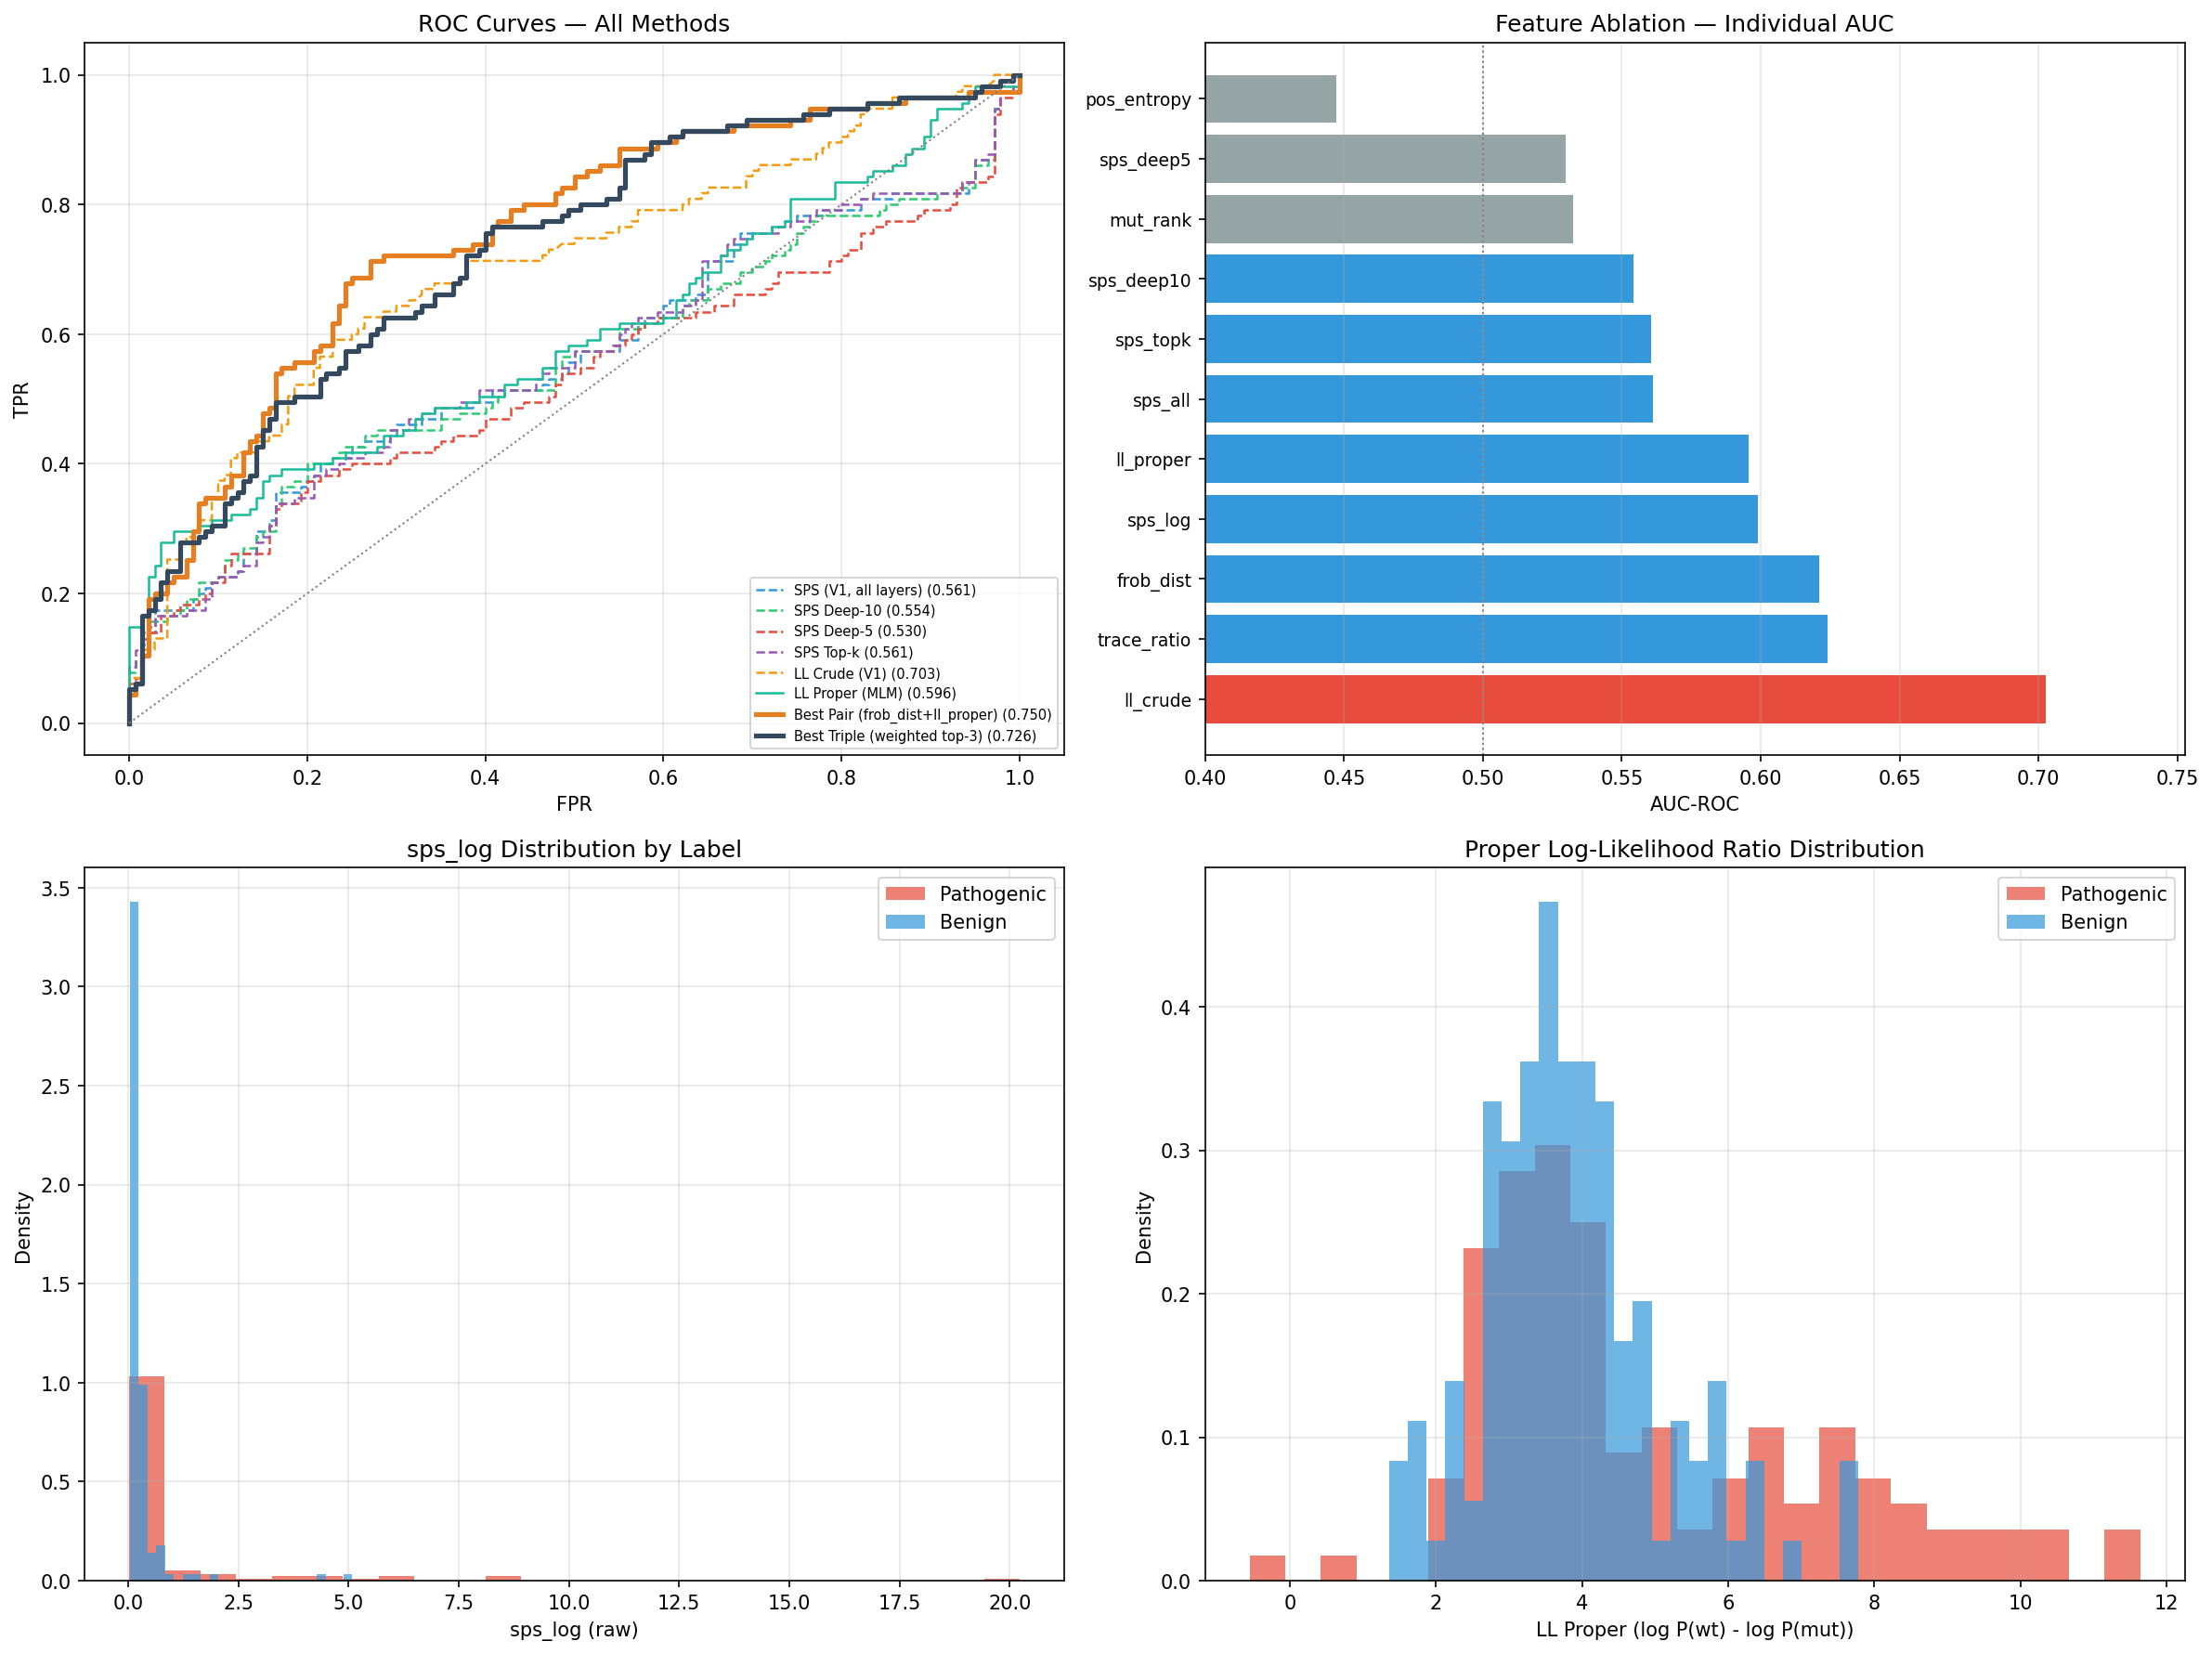
\includegraphics[width=0.91\textwidth]{../outputs/canonical/roc_tp53.png}
\caption{%
  \textbf{\methodname{} canonical TP53 results summary ($N$=255).}
  Best Pair (FrobDist+LL Proper, orange) reaches AUC=0.7498 and remains above
  all individual features and the Best Triple (black, 0.7264, rounded in the figure).
  Matrix-level features outperform eigenvalue-only SPS variants on TP53, while
  the proper-LL distribution is consistent with the bounded BRCA1 secondary
  transfer result (AUC=0.9174). Figure linked to canonical asset
  \texttt{outputs/canonical/roc\_tp53.png}; TP53 reproduces with
  $\Delta_{\text{rep}}$=0.0.
}
\label{fig:results}
\end{figure*}

% ============================================================================
\section{Discussion}\label{sec:discussion}
% ============================================================================

\methodname{} demonstrates that covariance geometry of PLM hidden states can
provide useful benchmark signal complementary to sequence-level log-likelihoods.

\textbf{Why feature complementarity works.}\;
The best TP53 result combines a spectral feature (FrobDist, geometric perturbation)
with a likelihood feature (LL Proper, evolutionary constraint).
These are mechanistically distinct: FrobDist measures how much the
\emph{shape} of the representation manifold changes, while LL Proper measures how
\emph{surprising} the mutant residue is.
Their complementarity suggests pathogenic mutations affect both the surface-level
amino acid preference and the deeper structural representation independently.

\textbf{Why LL Proper matters in the bounded BRCA1 transfer evaluation.}\;
Proper LL achieving AUC=0.9174 on the fixed BRCA1 subset despite 0.5956 on TP53
shows that this score remains informative in the secondary fixed-subset setting.
We keep the interpretation narrow: this bounded result does not establish
broader cross-protein behavior beyond the fixed BRCA1 subset evaluated here.

\textbf{Key findings:}
\begin{enumerate}[itemsep=1pt]
  \item \textbf{Matrix $>$ eigenvalue.}\;
    FrobDist/TraceRatio consistently outperform all SPS variants on TP53.
  \item \textbf{Feature complementarity.}\;
    Strongest TP53 classifier (0.7498) combines spectral geometry with
    masked-LM likelihood---neither is strongest alone.
  \item \textbf{Secondary BRCA1 bounded transfer evidence.}\;
    LL Proper: 0.9174 with zero retraining on the fixed subset.
  \item \textbf{TP53 canonical reproducibility.}\;
    $\Delta_{\text{rep}}$=0.0 under the repository's canonical execution path.
\end{enumerate}

\textbf{Limitations.}\;
Window size ($\pm$40), model size (150M), and mixing weights were not jointly
optimized.
SPS features remain weak (best: 0.5988); layer selection provided no improvement.
Evaluation limited to two proteins; ProteinGym~\cite{notin2023proteingym}
benchmarking with 87 proteins is future work.
Larger ESM2 variants (650M--15B) likely produce richer geometry.

% ============================================================================
\section{Reproducibility}
% ============================================================================

Seeds: 42 (PyTorch, NumPy, \texttt{random}).
This repository is distributed as a research reproducibility artifact anchored
to the TP53 canonical executable benchmark and a secondary bounded BRCA1
transfer evaluation without retraining.
Model: ESM2-150M (HuggingFace, public).
Dataset: ClinVar FTP (public).
$\Delta_{\text{rep}}$=0.0 for the TP53 canonical executable benchmark.
Code: \href{https://github.com/DaviBonetto/SpectralBio}{github.com/DaviBonetto/SpectralBio}.
Demo: \href{https://huggingface.co/spaces/DaviBonetto/spectralbio-demo}{huggingface.co/spaces/DaviBonetto/spectralbio-demo}.\par
Dataset: \href{https://huggingface.co/datasets/DaviBonetto/spectralbio-clinvar}{huggingface.co/datasets/DaviBonetto/spectralbio-clinvar}.

% ============================================================================
\section{Conclusion}
% ============================================================================

We presented \methodname{}, a zero-shot variant pathogenicity prediction framework
based on spectral analysis of PLM hidden-state covariance.
Matrix-level spectral features provide complementary signal to log-likelihood
ratios, yielding AUC=0.7498 on TP53 and
AUC=0.9174 on a secondary bounded transfer evaluation on a fixed BRCA1 subset
($N$=100) without retraining.
The consistent superiority of covariance-based features over eigenvalue-only
summaries suggests that full covariance structure may capture useful benchmark
signal underexplored by eigenvalue-only summaries.
These results are presented as a research reproducibility artifact with one
primary benchmark and one bounded secondary transfer evaluation.

\paragraph{Acknowledgments.}
Conducted under the Claw4S 2026 competition (Stanford--Princeton).
Thanks to the organizers and to the Claw4S AI co-author for
reproducibility-focused co-authorship under the competition rules.

% ============================================================================
\bibliographystyle{plainnat}
\begin{thebibliography}{5}
\footnotesize

\bibitem{lin2023evolutionary}
Lin, Z., Akin, H., Rao, R., et al.\ (2023).
Evolutionary-scale prediction of atomic-level protein structure with a language model.
\textit{Science}, 379(6637), 1123--1130.

\bibitem{meier2021language}
Meier, J., Rao, R., Verkuil, R., et al.\ (2021).
Language models enable zero-shot prediction of the effects of mutations on protein
function.
\textit{NeurIPS}, 34.

\bibitem{landrum2018clinvar}
Landrum, M.\,J., Lee, J.\,M., Benson, M., et al.\ (2018).
ClinVar: improving access to variant interpretations and supporting evidence.
\textit{Nucleic Acids Res.}, 46(D1), D1062--D1067.

\bibitem{bonetto2026spectralguard}
Bonetto, D.\ (2026).
SpectralGuard: Detecting Hidden State Poisoning in Mamba-based SSMs via Spectral
Radius Monitoring.
\textit{arXiv:2603.12414}.

\bibitem{notin2023proteingym}
Notin, P., Dias, M., Frazer, J., et al.\ (2023).
ProteinGym: Large-scale benchmarks for protein fitness prediction and design.
\textit{NeurIPS}, 36.

\end{thebibliography}

\end{document}
